\subsection{Lepton charge mis-identification}

\subsubsection*{Mechanisms}
The misidentification rate of leptons is governed by \\
\begin{align}
-\langle\frac{dE}{dx}\rangle \varpropto \frac{E}{m^2}
\end{align}
Thus this rate is significant for electrons and high energy ($E > 400GeV$) muons. Therefore only the electron charge misidentification is calculated. \\

Electron charge misidentification is due to:
\begin{enumerate}
\item Bremsstrahlung photon and conversion electron
\item Track misidentification
\end{enumerate}

Since a magnetic field exists within the detector, it is possible to infer the charge and momentum of electrons by the curvature of their tracks. However, there are cases when the reconstruction gives the wrong charge. 

\begin{figure}[h]
\centering
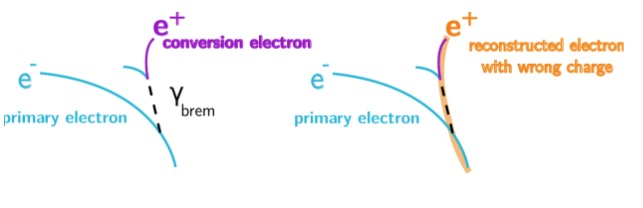
\includegraphics[width=\textwidth]{ChargeMisID/Brem}
\caption[Electron charge misidentification by bremsstrahlung]{Bremsstrahlung}
\label{fig:brem}
\end{figure}
\begin{figure}[h]
\centering
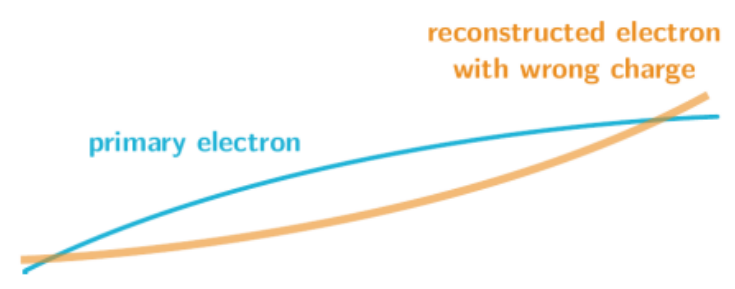
\includegraphics[width=\textwidth]{ChargeMisID/WrongTrack}
\caption[Electron charge misidentification by track mis-reconstruction]{Track mis-reconstruction}
\label{fig:wrong-track}
\end{figure}

\underline{Bremsstrahlung} \\
Charge misidentification may occur when an electron radiates a photon early in the detector (in the beampipe, or the first layers of the inner tracker). The radiated photon may then undergo pair production, and the converted electrons would leave tracks in the inner tracker.  One of these wrong tracks may then be matched to an energy deposit inside the calorimeter. In case the electron that left the track has the opposite charge to the original, then the charge inferred would be opposite to the charge of the original electron \cite{ElectronReco2011}. (Figure \ref{fig:brem}). 

The probability of bremsstrahlung increases with the amount of material the electron interacts with. Hence as the material budget of the detector changes with $|\eta|$ (Figure \ref{fig:material-budget}), it is expected that the charge misidentification rate ought to depend on  $|\eta|$.

\begin{figure}[h]
\centering
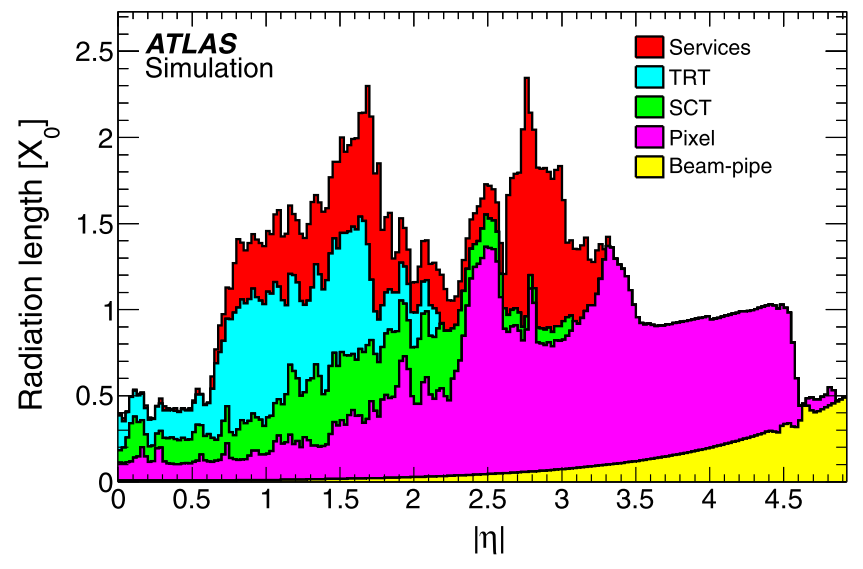
\includegraphics[scale=0.4]{ChargeMisID/Material-budget.png}
\caption[Amount of material traversed by a particle as a function of $|\eta|$]{Amount of material in front of the solenoid magnet and EM calorimeters traversed by a particle as a function of $|\eta|$. Figure from \cite{ElectronReco2011}.}
\label{fig:material-budget}
\end{figure}

\underline{Track mis-reconstruction}\\
Another possible source of charge misidentification is track mis-reconstruction. The near straight track of a high $p_T$ electron may be reconstructed with the opposite curvature, thus giving the opposite sign. (Figure \ref{fig:wrong-track})

\subsubsection*{Likelihood Method for Measuring Charge misID}
$Z\rightarrow e^\pm e^\mp$ events are studied for its relatively clean signal (see Figure \ref{fig:mll_ee_OS}) and because, by charge conservation,  the two daughter electrons of the $Z$ must be of opposite sign. In principle, if a $Z\rightarrow e^\pm e^\pm$ event is found, it must the case that the charge of one electron has been misidentified. The likelihood method was used to measure the charge misidentification rate. An alternative method, the tag-and-probe method, was also attempted; the results obtained were unsatisfactory. 

\begin{figure}[h]
\centering
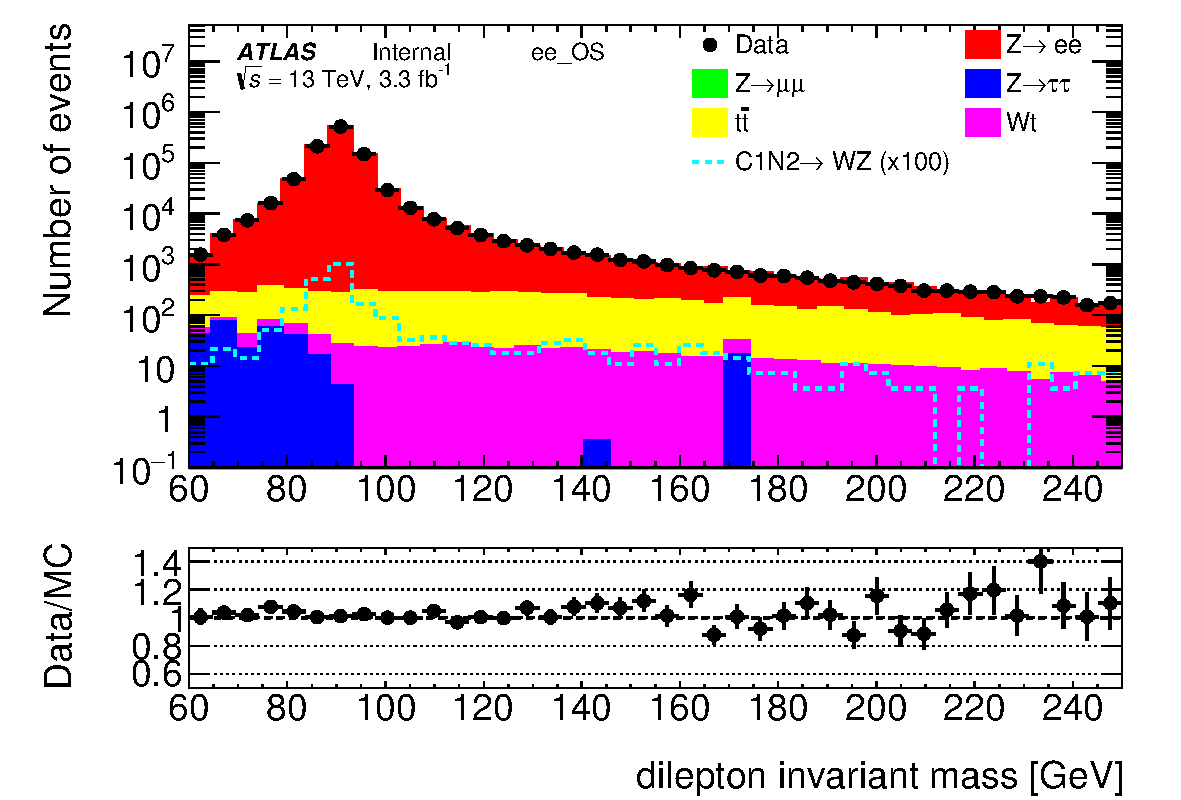
\includegraphics[scale=0.6]{ChargeMisID/mll_ee_OS.pdf}
\caption[Distribution of opposite-sign dielectron events]{Distribution of opposite-sign dielectron events. Note that the region near the Z mass $(91.2\ GeV)$ the signal is dominated by $Z\rightarrow e^\pm e^\mp$ events by at least 2 orders of magnitude. Plot by Lo Cheuk Yee, HKU.}
\label{fig:mll_ee_OS}
\end{figure}

The most likely rate of charge misidentification is determined by extremizing a likelihood function. 

$Z\rightarrow ee$ events were selected by imposing the following cuts:
\begin{itemize}
\item Events with two electrons
\item $75\ GeV < m_{ee} < 100\ GeV$
\item $\Delta \phi > 2$
\item Both same-sign and opposite-sign events are selected
\end{itemize}

The probability of observing a same sign event is:
\begin{equation}
p = P(e_1 \text{ correct sign})P(e_2 \text{ wrong sign}) + P(e_1 \text{ wrong sign})P(e_2 \text{ correct sign})
\end{equation}

Each electron is assigned a bin which depends on its $\eta$ and $p_T$. For events where one electron falls into bin $i$ and the other electron falls into bin $j$, the probability of observing a same-sign event is: 
\begin{equation}
p =(1-\epsilon_i)\epsilon_j + (1-\epsilon_j)\epsilon_i
\end{equation}
where $\epsilon_i$ is the charge misidentification rate in bin $i$.

The expected number of same-sign events is given by
\begin{equation}
N^{exp}_{SS} = np 
\end{equation}

A binomial distribution of observing $nss$ same-sign events is expected:
\begin{equation}
P(nss |\epsilon_i, \epsilon_j) =  C^n_{nss} p^{nss}(1-p)^{n-nss}
\end{equation}

Since $p$ is small, this can be approximated well by a Poisson distribution: 
\begin{equation}
P(nss |\epsilon_i, \epsilon_j) = \frac{(N^{exp}_{SS})^{nss} e^{-N^{exp}_{SS}}}{nss!}
\end{equation}

With this equation of the probability of observing $nss$ same-sign events given $\epsilon_i$ and $\epsilon_j$, the likelihood function of having $\epsilon_i$, $\epsilon_j$ given $nss$ observed same-sign events can be defined: 
\begin{equation}
L(\epsilon_i, \epsilon_j | nss) \equiv P(nss |\epsilon_i, \epsilon_j)
\end{equation}

For the likelihood across all combinations of bins $i,j$,
\begin{equation}
\mathcal{L} = \prod\nolimits_{i,j} L(\epsilon_i, \epsilon_j)
\end{equation}

By maxmizing the likelihood function, the most probable $\epsilon_i$, $\epsilon_j$ can be found for a given $nss$ observed same sign events. To simplify calculation, the logarithm function is applied to $\mathcal{L}$. To take advantage of the minimizer in ROOT, the negative of the function is minimized. 

The final function to be minimized is 

\begin{equation}
-\ln \mathcal{L} = -\sum\nolimits_{i,j} \Big\{ {nss}_{ij} \ln\big(n_{ij}[\epsilon_j(1-\epsilon_i) + \epsilon_i(1-\epsilon_j)]\big) - n_{ij}[\epsilon_j(1-\epsilon_i) + \epsilon_i(1-\epsilon_j)] - \ln (nss_{ij}!) \Big\}
\end{equation} 

\subsubsection*{Validation with Monte Carlo}
A Monte Carlo (MC) sample of simulated $Z \rightarrow ee$ events was used to develop and validate the likelihood algorithm. The information saved in the MC sample includes the \textit{truth} information of the simulated events, and the reconstructed event information produced from a detector simulator. 

%\footnote{MC sample used: \texttt{mc15\_13TeV:mc15\_13TeV.361106.PowhegPythia8EvtGen\_AZNLOCTEQ6L1\_Zee.merge.DAOD\_SUSY2.e3601\_s2576\_s2132\_r6765\_r6282\_p2419}} \todo{Fix this sample name. Should be included?}

For every reconstructed electron selected by the aforementioned conditions, an attempt was made to find the charge of the original daughter electron of Z. A reconstructed electron was first matched to a truth particle with the smallest $\Delta R = \sqrt{\Delta \phi^2 + \Delta \eta^2} < 0.1$ separation from the reconstructed electron. The truth particle was rejected if it was not an electron.\footnote{It could be the case that a hadron was misidentified as an electron \cite{ElectronReco2011}.} The decay path was then traversed upwards to find the original daughter electron of a Z boson. The truth particle was rejected if no Z boson was found in the path, or if the daughter particle of Z was not an electron.\footnote{It was found that sometimes the algorithm would match to a final-state radiation photon from Z.} An example of this algorithm is shown in Figure \ref{fig:find-daughter-electron}.

\begin{figure}[h!]
\centering
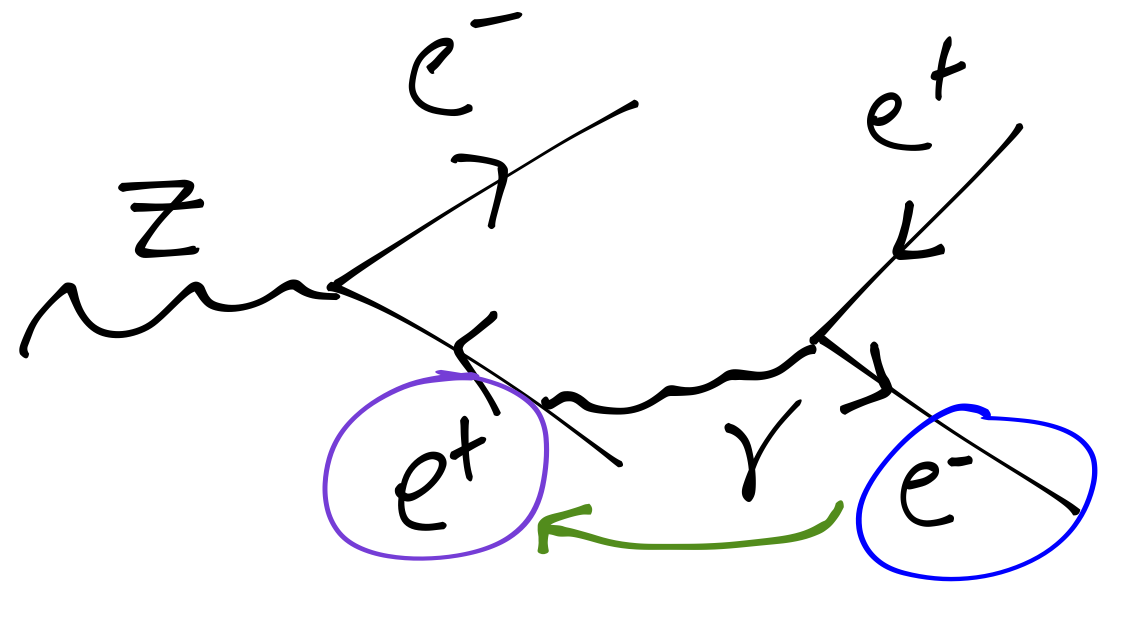
\includegraphics[scale=0.35]{ChargeMisID/MC-truth}
\caption[Finding the original daughter electron of Z]{Finding the  daughter electron of Z. The electron circled in blue is the truth electron matched to the reconstructed electron. The decay was traversed upwards to find the original daughter electron of a Z boson, circled in purple.}
\label{fig:find-daughter-electron}
\end{figure}

If the original electron daughter of Z was found, then it was considered to be the \textit{matched} electron of the reconstructed electron. If the charge of the matched electron was not identical to the charge of the reconstructed electron, then the charge was considered to be misidentified. Thus the true charge misidentification rate in each bin can be defined as:

\begin{equation}
\epsilon_{\text{MC}} = \frac{\text{Number of reconstructed electrons with charge opposite to its matched electron}}{\text{Total number of matched electrons}}
\end{equation}

\subsubsection*{Charge misID rates}
The charge misidentification rates of both LooseBaseline and Signal electrons were computed in bins of $|\eta|$ and $p_T$ (bin edges defined in Table \ref{table:binning}) by:
\begin{itemize}
\item the likelihood method on $3.2\  \text{fb}^{-1}$ of $pp$ collision data collected by ATLAS in 2015 (labeled in the plots as \textit{Data}),
\item the likelihood method on a $Z\rightarrow ee$ MC sample (labeled in the plots as \textit{MC LH}), and
\item extracting the true rates from the same MC sample (labeled in the plots as \textit{MC truth}).
\end{itemize}

\begin{table}[h!]
\centering
\begin{tabular}{c | c}
\textbf{Variable} & \textbf{Bin edges} \\
\hline
$|\eta|$ & 0, 0.5, 1, 1.37, 1.52, 1.8, 2.0, 2.5 \\
$p_T$ (GeV) &  20, 30, 40, 50, 60, 80, 120
\end{tabular}
\caption{Binning in $|\eta|$ and $p_T$}
\label{table:binning}
\end{table}

\begin{figure}[h!]
\centering
\subfloat[][Comparison of rates for LooseBaseline electrons]{\includegraphics[scale=0.39]{ChargeMisID/WoSub_loose/Pt.pdf}}
\subfloat[][Comparison of rates for Signal electrons]{
\includegraphics[scale=0.39]{ChargeMisID/WoSub_signal/Pt.pdf}}
\caption{Comparison of electron charge misidentification rates as a function of $p_T$}
\label{fig:rates-pt}
\end{figure}

\begin{figure}[h!]
\centering
\subfloat[][Comparison of rates for LooseBaseline electrons]{\includegraphics[scale=0.39]{ChargeMisID/WoSub_loose/Eta.pdf}}
\subfloat[][Comparison of rates for Signal electrons]{
\includegraphics[scale=0.39]{ChargeMisID/WoSub_signal/Eta.pdf}}
\caption{Comparison of electron charge misidentification rates as a function of $|\eta|$}
\label{fig:rates-eta}
\end{figure}



Figures \ref{fig:rates-eta} and \ref{fig:rates-pt} compare the rates  obtained by the above methods for all $p_T$ ranges over $|\eta|$ and for all $|\eta|$ ranges over $p_T$ respectively. The full two-dimensional histograms showing the rates obtained by each method are figures \ref{fig:ChargeMisID-loose} and \ref{fig:ChargeMisID-signal} while plots showing the comparison of rates in each bin are figures \ref{fig:chargeMisID-CompareLoose} and \ref{fig:chargeMisID-CompareSignal}.

In general, the rates measured on data increase with $|\eta|$, which is as expected because the material budget of the detector increases with $|\eta|$ (Figure \ref{fig:material-budget}). 

The rates also rise gradually with $p_T$, which corresponds to electrons having straighter tracks, and thus a higher probability of being reconstructed with the wrong direction of curvature. There is an exception to this trend at $p_T\sim45$ GeV.

The rates obtained by the likelihood method on data and MC follow the same trends and generally agree with each other within reasonable limits. The differences can be attributed to the differences between the MC simulation and actual conditions inside the detector.

Figures \ref{fig:rates-eta} and \ref{fig:rates-pt} seem to suggest that the agreement between the MC truth and likelihood on MC do not agree well in all bins, especially at low $p_T$. However, further investigation into the comparisons in individual $|\eta|$ and $p_T$ bins show that they do, in fact, agree within reasonable limits. Thus the likelihood-based algorithm developed is shown to operate reasonably well and  provides reliable measurements when applied to data.

\newcommand{\TwoD}[2]{
  \makebox[\textwidth][c]{
  \begin{minipage}{1.15\textwidth}
  \subfloat[][#2]{\adjustbox{trim={0.02\width} {0.01\height} 0 {0.06\height},clip}%
    {\includegraphics[width=\textwidth]{#1}}
    }
  \end{minipage}} 
}

\begin{figure}[h]
\centering
\TwoD{ChargeMisID/WoSub_loose/hData.pdf}{Rates from likelihood on data}
\end{figure}

\begin{figure}[h]
\ContinuedFloat
\centering
\TwoD{ChargeMisID/WoSub_loose/hMCLH.pdf}{Rates from likelihood on MC}
\end{figure}

\begin{figure}[h]
\ContinuedFloat
\centering
\TwoD{ChargeMisID/WoSub_loose/hMC.pdf}{Rates from MC truth}
\caption{Charge misidentification rates for LooseBaseline electrons}
\label{fig:ChargeMisID-loose}
\end{figure}

\begin{figure}[h]
\centering
\TwoD{ChargeMisID/WoSub_signal/hData.pdf}{Rates from likelihood on data}
\end{figure}

\begin{figure}[h]
\ContinuedFloat
\centering
\TwoD{ChargeMisID/WoSub_signal/hMCLH.pdf}{Rates from likelihood on MC}
\end{figure}

\begin{figure}[h]
\ContinuedFloat
\centering
\TwoD{ChargeMisID/WoSub_signal/hMC.pdf}{Rates from MC truth}
\caption{Charge misidentification rates for Signal electrons}
\label{fig:ChargeMisID-signal}
\end{figure}

\begin{figure}[h]
\centering
\subfloat{
  \subfloat{\includegraphics[page=1,scale=0.25]{ChargeMisID/WoSub_loose/EtaPt.pdf}}
  \subfloat{\includegraphics[page=2,scale=0.25]{ChargeMisID/WoSub_loose/EtaPt.pdf}}
  \subfloat{\includegraphics[page=3,scale=0.25]{ChargeMisID/WoSub_loose/EtaPt.pdf}}
}

\subfloat{
  \subfloat{\includegraphics[page=4,scale=0.25]{ChargeMisID/WoSub_loose/EtaPt.pdf}}
  \subfloat{\includegraphics[page=5,scale=0.25]{ChargeMisID/WoSub_loose/EtaPt.pdf}}
  \subfloat{\includegraphics[page=6,scale=0.25]{ChargeMisID/WoSub_loose/EtaPt.pdf}}
}

\subfloat{
  \subfloat{\includegraphics[page=1,scale=0.25]{ChargeMisID/WoSub_loose/PtEta.pdf}}
  \subfloat{\includegraphics[page=2,scale=0.25]{ChargeMisID/WoSub_loose/PtEta.pdf}}
  \subfloat{\includegraphics[page=3,scale=0.25]{ChargeMisID/WoSub_loose/PtEta.pdf}}
}

\subfloat{
  \subfloat{\includegraphics[page=5,scale=0.25]{ChargeMisID/WoSub_loose/PtEta.pdf}}
  \subfloat{\includegraphics[page=6,scale=0.25]{ChargeMisID/WoSub_loose/PtEta.pdf}}
  \subfloat{\includegraphics[page=7,scale=0.25]{ChargeMisID/WoSub_loose/PtEta.pdf}}
}
\caption[Comparison of charge misidentification rates for LooseBaseline electrons]{Comparison of charge misidentification rates for LooseBaseline electrons}
\label{fig:chargeMisID-CompareLoose}
\end{figure}

\begin{figure}[h]
\centering
\subfloat{
  \subfloat{\includegraphics[page=1,scale=0.25]{ChargeMisID/WoSub_signal/EtaPt.pdf}}
  \subfloat{\includegraphics[page=2,scale=0.25]{ChargeMisID/WoSub_signal/EtaPt.pdf}}
  \subfloat{\includegraphics[page=3,scale=0.25]{ChargeMisID/WoSub_signal/EtaPt.pdf}}
}

\subfloat{
  \subfloat{\includegraphics[page=4,scale=0.25]{ChargeMisID/WoSub_signal/EtaPt.pdf}}
  \subfloat{\includegraphics[page=5,scale=0.25]{ChargeMisID/WoSub_signal/EtaPt.pdf}}
  \subfloat{\includegraphics[page=6,scale=0.25]{ChargeMisID/WoSub_signal/EtaPt.pdf}}
}

\subfloat{
  \subfloat{\includegraphics[page=1,scale=0.25]{ChargeMisID/WoSub_signal/PtEta.pdf}}
  \subfloat{\includegraphics[page=2,scale=0.25]{ChargeMisID/WoSub_signal/PtEta.pdf}}
  \subfloat{\includegraphics[page=3,scale=0.25]{ChargeMisID/WoSub_signal/PtEta.pdf}}
}

\subfloat{
  \subfloat{\includegraphics[page=5,scale=0.25]{ChargeMisID/WoSub_signal/PtEta.pdf}}
  \subfloat{\includegraphics[page=6,scale=0.25]{ChargeMisID/WoSub_signal/PtEta.pdf}}
  \subfloat{\includegraphics[page=7,scale=0.25]{ChargeMisID/WoSub_signal/PtEta.pdf}}
}
\caption[Comparison of charge misidentification rates for Signal electrons]{Comparison of charge misidentification rates for Signal electrons}
\label{fig:chargeMisID-CompareSignal}
\end{figure}

\FloatBarrier
